\documentclass[10pt, conference, compsocconf]{IEEEtran}
\usepackage[nocompress]{cite}
\usepackage[font=normalsize,labelfont=sf,textfont=sf]{subfig}
\usepackage{graphicx}
\usepackage{arabtex}
\usepackage[cmex10]{amsmath}
%\usepackage{flushend}

\begin{document}

\title{Fast Classification of Handwritten On-line Arabic Characters}

\author{\IEEEauthorblockN{George Kour}
\IEEEauthorblockA{Faculty of Engineering\\
Tel-Aviv University\\
Tel-Aviv Jaffa, Israel\\
Email: georgeko@post.tau.ac.il}
\and
\IEEEauthorblockN{Raid Saabne}
\IEEEauthorblockA{Department of Computer Science\\
Tel Aviv-Yaffo Academic Collage, Israel\\
Triangle R\&D Center, Kafr Qara, Israel\\
Email: saabni@cs.bgu.ac.il}
}


\maketitle

\begin{abstract}
Delaying the analysis launch until the completion of the handwritten word scribing, restricts on-line recognition systems to meet the highly responsiveness demands expected from such applications, and prevents implementing advanced features of input typing such as automatic word completion and real-time automatic spelling.
This paper proposes an efficient Arabic handwritten characters recognizer aimed at facilitating real-time handwritten script analysis tasks.
The fast classification is enabled by employing an efficient embedding of the feature vectors into a normed wavelet coefficients domain in which the Earth Movers Distance metric is approximated using the Manhattan distance.
A sub-linear time character classification is achieved by utilizing metric indexing techniques.
Using the results of the top ranked shapes of each predicted character, a list of candidate shapes of Arabic word parts is generated in a filter and refine approach to enable fast yet accurate recognition results in a dictionary-free environment.
The system was trained and tested on characters and word parts extracted from the ADAB database, and promising accuracy and performance results were achieved.\\
\end{abstract}

\begin{IEEEkeywords}
Arabic character recognition; handwriting recognition; on-line script recognition; real-time handwriting segmentation;
\end{IEEEkeywords}

\section{Introduction}
The growing use of keyboard-less electronic devices, and the fact that handwriting remains a commonly used mean for information recording, gave rise to a significant increase in interest in on-line handwriting recognition in recent years.

The Arabic script is written from right to left in a semi-cursive manner in both printed and handwritten forms. 
Most letters are written in four different letter shapes depending on their position in the word.
Among the basic letters, six are dis-connective which do not connect to the following letter and have only two shapes each. 
The presence of dis-connective letters interrupts the continuity of the graphic form of a word and closes the \emph{word part} (WP).

Considerable amount of work has been done in the area of Arabic character recognition but with limited success, this is due to the unconstrained nature of Arabic characters and the large variety of writing styles.
The nature of the Arabic handwriting requires the letters classification system to be trained over a large set of samples that cover the large variation of letters forms.
Similarity measure techniques that imitate the human intuition, such as the well known \emph{Dynamic Time Warping} (DTW) and the \emph{Earth Mover's Distance} (EMD), are computationally expensive and may take more than a few hours to find, for a given query object, the most similar objects in a large sample set, on an average personal computer.
A well known technique for achieving a speed-up is by embedding the compared objects into a space equipped with an efficient metric that approximates the distance function in the original space.

The cursiveness of the Arabic script, supposedly requires delaying the launch of the recognition process until the completion of the word scribing.
However, a recognition-based segmentation approach, proposed in \cite{kour2014real}, demonstrated the feasibility of segmenting strokes while being handwritten.
Morphological features were employed to nominate potential segmentation points. 
The sub-strokes induced by the segmentation points is recognized using the classifier presented in this paper.
The character candidates and their similarity scoring is saved in a scoring matrix, where the cell ${i,y}$ contains the classification information of the sub-stroke spanning from the potential segmentation point $i$ to the potential segmentation point $j$.
The final segmentation points are then selected by finding the best-scored segmentation path in the scoring matrix. 
The real-time nature of the segmentation technique required the characters classifier to be extremely fast.
In this paper we present the implementation of the efficient characters classifier.

%The classifier employs a linear time embedding algorithm for approximating EMD \cite{shirdhonkar2008approximate} to transform the feature vectors to a normed space and facilitate the use of fast nearest neighbours search techniques.
%Then, a $k$-NN classifier is used to produces a short list of candidates enabling us to apply expensive matching methods, such as DTW, yet keep sub-linear searching time.

The rest of the paper is organized is follows. 
In Section \ref{sec:related_work} we mention related works. 
The character classifier is described in Section \ref{sec:approach}. 
In Section \ref{sec:samples_collection} we describe the letter samples extraction from the ADAB database.
The system results are discussed in Section \ref{sec:experimental_results}.
In Section \ref{sec:wps_recognition}, we utilize the resulted segmentation and letters classification information provided by the real-time segmentation technique, proposed in \cite{kour2014real}, to improve the performance of a later holistic recognition process.
Summary and future direction, are presented in Section \ref{sec:summary_future_work}. 

\section{Related Work}
\label{sec:related_work}
Literature in the field of cursive handwriting recognition has established two main approaches. 
First, the holistic approach, which considers the global properties of the written text and recognizes the input word shape as a whole \cite{biadsy2011segmentation, saabni2009hierarchical}. 
While having many advantages, the holistic approach requires the classifier to be trained over the entire dictionary, which is impractical for large dictionaries (containing more than 20,000 words) \cite{elanwar2012unconstrained}.
The second approach is the analytic approach, which involves segmenting words into individual characters and then classifying each character \cite{abdulla2008off, sari2002off, Dinges2011}. 
Methods that follows this approach require a reliable character classifier to correctly segment and recognize the handwritten script.

One of the earliest studies in the field of on-line Arabic character recognition was carried out by El-Wakil and Shoukry in 1989 \cite{el1989line}.
Many types of classification techniques were investigated since then, including Artificial Neural Networks \cite{alijla2012oiahcr,ismail2012online}, Decision Trees \cite{ismail2012online, al2010recognition, omer2010online}, Hidden Markov Models \cite{biadsy2006online} and $k$-NN \cite{elglaly2011isolated}.
An on-line Arabic handwritten character recognition method, which uses structural features and decision trees, was presented by Al-Taani and Al-Haj \cite{al2010recognition}. 
The system was tested on a set of 1400 different characters and achieved about 75\% recognition rate. 
The dataset was obtained by capturing the handwriting of ten users that wrote the 28 Arabic characters, in their isolated form, five times in order.
A rules based approach for on-line Arabic characters classification was proposed in \cite{ismail1859online}. 
The performance of the system was compared to the classification results obtained using artificial neural networks and and decision trees. 
A set of 504 characters were used for training and the test set contained 336 characters. 
The system obtained a recognition rate of about 97\%. 
Addakiri and Bahaj \cite{addakiri2012line} presented an on-line Arabic handwritten character
recognition system based on Neural Networks. 
Their approach was tested on 1400 different characters written by ten users and achieved accuracy of 83\%.

EMD is a natural and intuitive metric to measure similarity between histograms. 
It has been successfully used in many fields of image matching and retrieval \cite{grauman2004fast, rubner2000earth}.
However, it subjected to a high computational complexity.
Nevertheless, a significant speed-up can be achieved by using embedding techniques.
Much work has been done on embedding the EMD metric into a normed space, usually into the $l_p$ norm, in order to facilitate efficient and fast nearest neighbour extraction using indexing techniques \cite{bourgain1985lipschitz}. 
The efficient embedding of the EMD metric proposed by \cite{shirdhonkar2008approximate} to a normed space has been used in \cite{saabni2013efficient} for efficient word image retrieval.

\section{Our Approach}
\label{sec:approach}
In the presented work, we propose a fast and accurate classification technique for handwritten Arabic characters.
In Figure \ref{fig:letters_classifier_learning_flow} we give a high level flow visualization of the classification system.
The classifier receives a sequence of points $S=\{p_{i}\}_{i=1}^{n}$ representing the letter trajectory and a letter position $\phi \in \{Ini, Mid, Fin, Iso\}$.
The query sequence goes through several stages that include preprocessing, feature extraction, embedding, dimensionality reduction and eventually a classification process that outputs a short list of candidates and their scoring, which indicates the perceptual similarity between the sequence and the candidates. 
Each stage will be discussed in details in the following subsections.

\begin{figure}
\centering
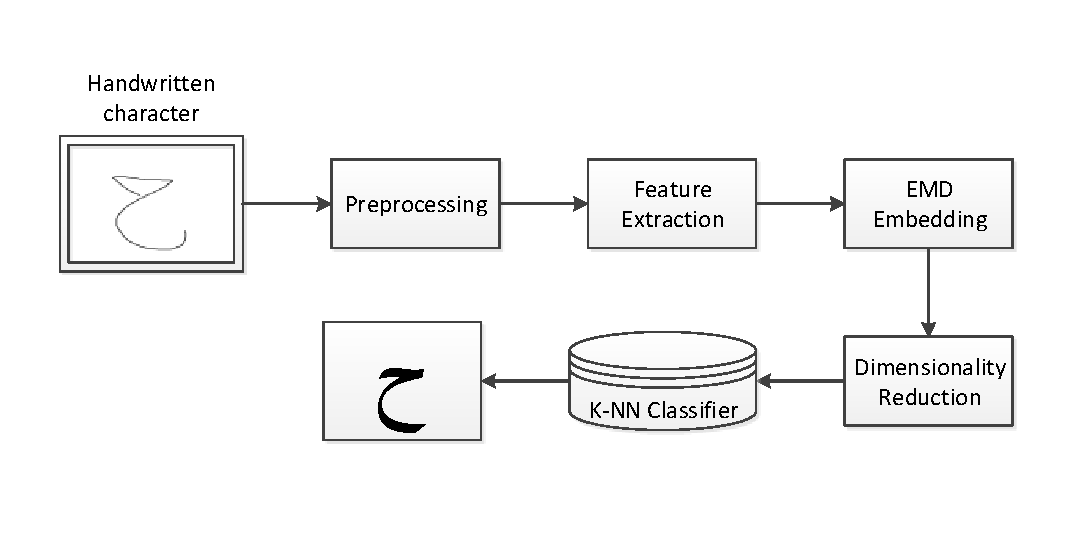
\includegraphics[width=1\columnwidth]{./figures/letters_classifier_learning_flow2}       
\caption{High level diagram of the classification process.}
\label{fig:letters_classifier_learning_flow}
\end{figure}
 
\subsection{Preprocessing}
Digitizers tend to generate a jagged and non-uniform sampling of the trajectory scribed on their surface, therefore, preprocessing operations are usually needed to impose certain uniform structure on the data, to comply with the structure required by the subsequent parts of the system \cite{al2011online}. 
The preprocessing stage consists of three methods: \emph{normalization}, \emph{noise elimination} and \emph{re-sampling}.

Size normalization is performed to achieve a uniform size of the bounding box surrounding the pattern so that it will fit into a $[0,1]\times[0,1]$ bounding box without affecting the original aspect ratio. 

Then, the \emph{Douglas-Peucker Polyline Simplification algorithm} \cite{douglas1973algorithms} is employed for eliminating points duplication and inadequacies caused by hand vibrations. 
It reduces the number of vertices in a piecewise linear curve.
Given a pre-set tolerance parameter $\varepsilon$, it outputs a simplified curve which contains a subset of the points on the original curve.
In this work the tolerance parameter $\varepsilon$ was empirically set to ${1 \over 75}$.

The simplification process produces a highly angular, and non-uniform distribution of points along the stroke trajectory.
This step, using splines interpolation, aims at producing an equidistant smoothed data sequence, given a re-sampling target number of points $R$, which was set to 40. 
Given a stroke $S=\{(x_i,y_i)\}_{i=1}^{n}$, let $f_{x}(d)$ and $f_{y}(d)$ be the quadratic piecewise interpolation functions of $\{x_i\}_{i=1}^{n}$ and $\{y_i\}_{i=1}^{n}$, respectively. 
$f_{x}(d)$ and $f_{y}(d)$ are functions of the coordinate values with respect to the arc-length distance from the pattern's starting point. 
Let $t_i=i\frac{L}{R}$ for $i=0,...,R$ where $L$ is the arc-length of the pattern.
The re-sampled sequence is given as follows:
\begin{equation}
\widehat{S}=\{(f_x(t_i),f_y(t_i))\}_{i=1}^{R}
\end{equation}

Figure \ref{fig:before_after_preprocessing} visually demonstrates the resulting sequence after applying each step in the preprocessing stage on a trajectory sequence of the letter \RL{b}. 

\begin{figure}
	\centering
        \subfloat[]{
            \label{fig:preprocessing_orig}
            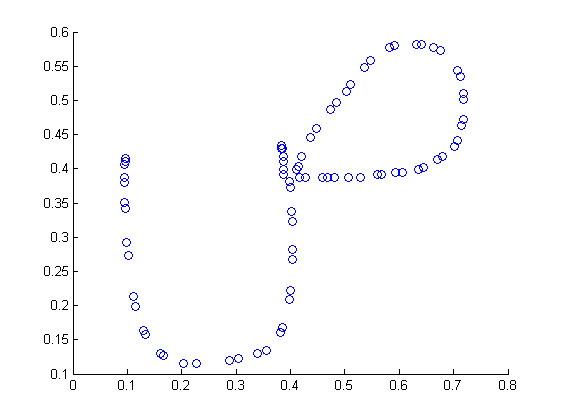
\includegraphics[width=0.5\columnwidth]{./figures/preprocessing_orig}
        }
        \subfloat[]{
           \label{fig:preprocessing_norm}
           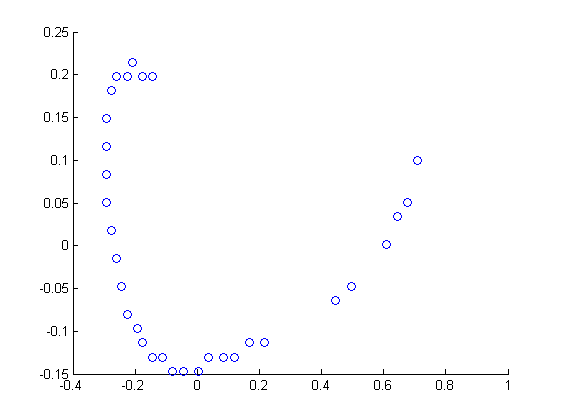
\includegraphics[width=0.5\columnwidth]{./figures/preprocessing_norm}
        }  \\
        \subfloat[]{
            \label{fig:preprocessing_simpl}
            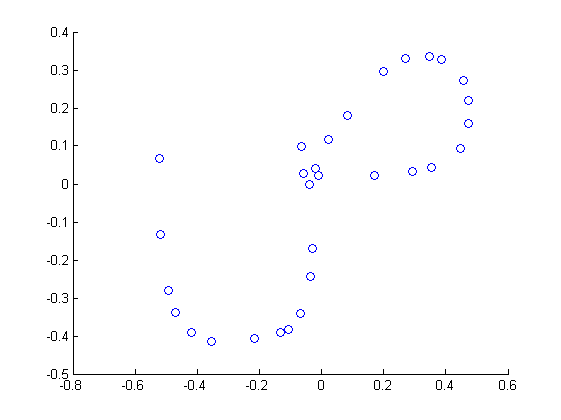
\includegraphics[width=0.5\columnwidth]{./figures/preprocessing_simpl}
        }
        \subfloat[]{
           \label{fig:preprocessing_resamp}
           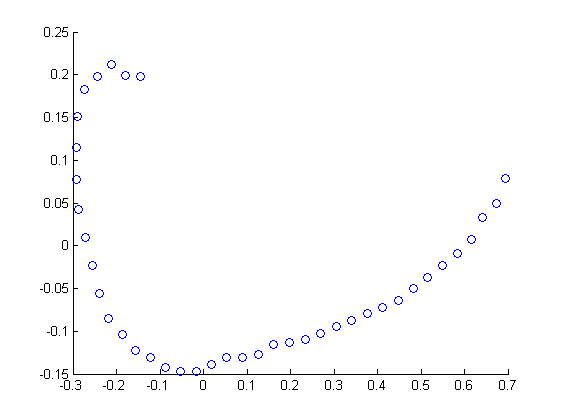
\includegraphics[width=0.5\columnwidth]{./figures/preprocessing_resamp}
        }
    \caption{A sample of the letter \RL{b} before preprocessing (a); after normalization (b); after noise elimination (c) and after re-sampling (d).}
   \label{fig:before_after_preprocessing}
\end{figure}

\subsection{Features Extraction}
Two shape descriptors were employed in this work, the \emph{Shape Context} (SC) \cite{belongie2002shape} and the \emph{Multi Angular Descriptor} (MAD) \cite{saabni2013multi}.
The SC descriptor has been proved to be an efficient feature for shapes matching.
Given a sequence of points $S=\{p_i\}_{i=1}^n$, the descriptor of the point ${p_i}$, is the coarse histogram of the relative coordinates.
MAD captures the angular view to multi resolution rings in different heights. 
The shape is treated as a two dimensional set of points and the different rings are upper view points from rings around the shape centroid with different sizes and heights. 
To enable scale and translation invariance, the radius and height of these rings are calculated using the diameter and centroid of the shape.

\subsection{The Earth Mover's Distance Embedding}
Histogram based descriptors, such as the shape context, are in many cases compared using a bin-wise dissimilarity techniques such as the Euclidean distance or the $\chi^2$ statistic.
While such dissimilarity measures can be computed very fast, they usually fail to consider local and global small variations. 
These variations, which would be perceived as minor by a human, may result in a large dissimilarity value between two histograms. 
Generally speaking, the distance between two histograms can be viewed as a special case of the well-known \emph{transportation problem}, a.k.a the \emph{Monge-Kantorovich problem} \cite{rachev1985monge}.
The \emph{Earth Mover's Distance} (EMD), introduced by Rubner et al. in \cite{rubner2000earth}, is a solution to the transportation problem which was experimentally verified to capture well the perceptual notion of a difference between images \cite{grauman2004fast}.

Given two distributions, one can be seen as piles of sand and the other as a collection of holes. 
EMD measures the least work needed to fill the holes with sand taken from the piles, where a unit of work corresponds to the transporting a unit of sand from the pile to the hole depending on their distance.
The main impediment for using EMD is its $O\left( {{N^3}\log N} \right)$ computational complexity (for an $N$-bin histogram). 
Thus, searching for similar shapes (nearest neighbours) in a large database, is almost impractical since a linear scan of the database would require computing a comparison of super-polynomial complexity for each database member against the query shape \cite{saabni2013efficient}. 

Greatly reducing the EMD calculation time can be achieved using metric approximation techniques.  
Several approximation algorithms have been proposed to speed-up the computation of EMD. 
Indyk and Thaper \cite{indyk2003fast} presented a technique for embedding the un-normed EMD metric into the $L_1$ space so that the EMD distance between the two objects is comparable to the Manhattan distance between the two points which represent the embedding of the two objects.
Their method was used by Grauman and Darrell \cite{grauman2004fast} for contour based shape matching.
In a subsequent work done by Shirdhonkar and Jacobs \cite{shirdhonkar2008approximate}, the authors proposed a linear time method for approximating the EMD between two histograms using the weighted wavelet coefficients of the difference histogram. 
It is done by calculating the $L_1$ norm of the coefficients vector of the embedding as given in Equation \ref{eq:emd_embedding}.
\begin{equation}
d(p)_{wemd}= \sum\limits_{\lambda} 2^{-j(1+n/2)}|p_{\lambda}|
\label{eq:emd_embedding}
\end{equation}
where $p$ is the n-dimensional difference histogram and $p_{\lambda}$ is the wavelet transform coefficients. 
The index $\lambda$ includes both shifts and the scale j.
Intuitively, the wavelet transform splits up the difference histogram according to scale and location where each coefficient represents the solution to the EMD subproblem. 
For a single wavelet, the mass to be moved is proportional to the volume of $|\psi_j(x)|$, i.e., to $2^{-jn/2}$ and the distance to be travelled is proportional to the span of the wavelet, namely $2^{-j}$. The sum of all distances is an approximation to EMD, as formally defined in Equation \ref{eq:emd_embedding}. 
This can be viewed as similar to the way packages are shipped over large distances. 
The route is broken into several pieces which are large and small distances. 
Packages from nearby places are merged at the end of the short distance route piece to travel together. 
Then another merge is done of packages from the entire country to be shipped together to the destination country. 
The sum of the distances travelled is an approximation to the actual distance.
Th can be computed in $O\left( N \right)$ time complexity.

In this work, we have used the embedding proposed by Shirdhonkar and Jacobs and evaluated several wavelets, including the Haar wavelet, the Coif-let of order 1, the Coif-let of order 2 and the Symlets of order 5 wavelets.
The Haar wavelet achieved the best classification results.

\subsection{Dimensionality Reduction}
\label{subsec:dimensionality_reduction}
Dimensionality reduction is the process of reducing the number of variables taken into consideration in order to avoid practical complications and performance issues. 
Ideally, the reduced representation should have a dimensionality that corresponds to the intrinsic dimensionality of the data which is the minimum number of parameters needed to account for when classifying an unlabelled sample \cite{van2009dimensionality}.
The need for employing dimensionality reduction in this work emerged from the sparse vectors produces by the EMD embedding of the feature vectors into the wavelet coefficient domain.
For instance, when we used the shape context descriptor and the Haar wavelet, the embedding produced sparse vectors in $\mathbf{R}^{2422}$. 

\emph{Principle component analysis} (PCA) followed by \emph{linear discrimination analysis} (LDA) is a commonly used technique in fields where the feature space is highly dimensional, exploiting the efficiency of PCA and the discrimination power of LDA \cite{yu2001direct,yang2003can}.
The major drawback of the PCA is that it is an unsupervised technique, namely, it does not take into consideration the labelling information of the data and heavily rely on the assumption that most information is contained in those directions where input data variance is maximal.
On the contrary, \emph{Linear Discrimination Analysis} (LDA) is a supervised technique performing dimensionality reduction while preserving as much of the class discriminatory information as possible \cite{fisher1936use}. 

The dimensionality reduction process starts by projecting the embedded vectors into the PCA space where the target dimensionality, i.e., the number of principal components taken into consideration, is the minimal to achieve data preservation rate of 98\%.
As seen in Table \ref{table:dr_dimensions_results}, the dimensionality was reduced by PCA in two orders of magnitude.

Since there is a large variation in handwritten letters in the Arabic script, the grouping different perceptual shapes in a single class would negatively affect the LDA.
Thus, before applying LDA, each character class was partitioned into four clusters, using $L_1$-k-medoids algorithm, and for each cluster a unique sub-label was assigned. 
This sub-labelling was then used by the LDA, where the target number of dimensions was estimated using the \emph{maximum likelihood estimation} method described in \cite{levina2004maximum}.

\begin{table}
\centering
\renewcommand{\arraystretch}{1.2}
\begin{tabular}{ | c | c | c | c |}
\hline
\textbf{Letter position} & \textbf{Number of samples} & \textbf{PCA} & \textbf{PCA+LDA}\\
\hline                 
  Ini & 1405 & 48 & 9 \\ 
  \hline
  Mid & 1196 & 52 & 10 \\ 
  \hline
  Fin & 1629 & 44 & 9 \\ 
  \hline
  Iso & 1372 & 39 & 8 \\ 
  \hline
\end{tabular}
\caption{The dimensionality of the four datasets after applying PCA and PCA+LDA.}
\label{table:dr_dimensions_results} 
\end{table}

\subsection{Metric Indexing and Candidates Re-Scoring}
\label{subsec:candidates_rescoring}
The embedding of the sample set into a normed space facilitates the usage of metric indexing methods, such as k-d trees \cite{bentley1975multidimensional}, and approximate k-NN techniques such as Locality Sensitive Hashing (LSH) \cite{gionis1999similarity}.
Such techniques, solve the problem of searching $k$-NN in a large set and avoid linear scan of the entire dataset.
In our implementation we preferred to use the k-d tree since it returns the exact nearest neighbours and because the dimensionality of the data after dimensionality reduction is small.

Given an unlabelled sequence $q$, the $k$-NN classifier returns a set of $k$ potential letter candidates from the sample set, scored using their distance from $q$ in the coefficient wavelet domain.
In our implementation $k=10$.
The scoring of the candidates can be conducted by calculating the distance of a candidate to the query object in the reduced embedded space, using the Manhattan distance.
This will give the approximate EMD distance between them. 
However, in implementations that require exact scoring of the candidates, the approximated EMD distance may not be sufficient and an additional scoring stage should be employed to obtain a more accurate similarity measure between the query object and the candidates.
Nevertheless, in most cases such similarity measure technique are computationally expensive can be applied only on a short list of candidates rather than on the entire sample set.
In this work, re-scoring of the candidates is done by calculating the DTW distance between the preprocessed sequence of the query letter and each one of the candidates.
The constrained version of DTW using the Sakoe-Chuba Band \cite{sakoe1978dynamic} demonstrated better results the unconstrained version of DTW.

\section{Samples Collection}
\label{sec:samples_collection}
The character samples used in this work were extracted from the ADAB database \cite{el2009icdar}, a standard database of on-line Arabic handwriting script. 
It is freely available and consists of more than 20k Arabic handwritten words (937 Tunisian town/village names) scribed by more than 170 different writers. 
A manual segmentation of the word samples was required to extract letter samples \cite{kour2014real}.
The characters distribution with respect to their position is given in Table \ref{table:dr_dimensions_results}.
The extracted set was used for both training the system and testing the performance of the classifier as detailed in the subsequent section.

In the Arabic handwriting, there are cases in which two letters are vertically connected, i.e., are not connected using a horizontal ligature.  
Such composite characters are usually difficult to be separated by the segmentation system and are treated as a single letter.
In this work we considered the following combinations as composite characters: \RL{l.h-} , \RL{lm-} and \RL{lA}.

\section{Experimental Results}
\label{sec:experimental_results}

The system was implemented and tested using the Matlab environment.
The accuracy and the time performance of the classifier was measured using 10-fold cross-validation.
Using a public and not a self collected samples gives our results a further firmness.
In Table \ref{table:results_position}, the Correct Classification Rate (CCR), recall and precision rates are given for each characters position.
The last row in Table \ref{table:results_position} shows the accumulative average of the results weighted according to the amount of samples in each dataset.

\begin{table}
\centering
\renewcommand{\arraystretch}{1.2}
\begin{tabular}{ | c | c | c | c | c |}
\hline
	\textbf{Character Position} & \textbf{CCR} & \textbf{Recall} &  \textbf{Precision} \\
	\hline 
	Ini & 92\% & 97\% & 97\% \\                
  	\hline
  	Mid & 89\% & 85\% & 90\% \\
  	\hline
  	Fin & 91\% &  95\% & 100\% \\
  	\hline
  	Iso & 92\% &  91\% & 95\% \\
  	\hline
  	\textbf{Overall} & \textbf{91\%} &  \textbf{93\%} & \textbf{96\%} \\
  	\hline
\end{tabular}
\caption{Classification results by character position.}
\label{table:results_position} 
\end{table}

In Table \ref{table:configurations} we propose several activation configurations of the presented approach that target different balance points between accuracy and time performance.
In each experiment, the classifier performance was measured in terms of accuracy and the average response time for classifying a single sample.
The first configuration, titled \emph{High Accuracy}, we evaluate the classifier as presented in this work, including the re-scoring stage described in Section \ref{subsec:candidates_rescoring}.
Applying the re-scoring, although being invoked on a short list of candidates, ten candidates in our implementation, has a considerable impact on the classifier time performance. 
This configuration should be used in implementations which require high classification rate and can tolerate a certain degree of latency.
In the second configuration, named \emph{Low Latency}, the re-scoring stage is skipped.
This configuration should be considered in cases where the time performance is a critical factor, such as in real-time classification and recognition-based script segmentation systems.
When the top three candidates is considered, the difference in accuracy is small between the first and second configurations, and the latency resulted from the re-scoring done in the first configuration, in most cases, will not pay. 
The dimensionality reduction and the indexing processes are both computationally expensive and time consuming. 
Although both stages are usually performed off-line in the learning stage, in systems where the learning is performed on-line, the latency they impose on the learning process is undesired.
Thus, in the third configuration, named \emph{Fast Learning}, both the dimensionality reduction and the indexing stages were omitted from the learning process.
In addition, no re-scoring is performed in the classification flow.
Comparing the results of the this configuration with the second experiment shows that the dimensionality reduction process done in the second configuration has improved the time performance of the classifier significantly, without affecting much the classification rate.
We have noted that the vast majority of the delay was caused by the dimensionality reduction stage.
However, due to the sensitivity of the k-d tree to high dimensional data, when omitting the dimensionality reduction process, one should not perform indexing using k-d tree because it would negatively affect the classification repose time.
Skipping the dimensionality reduction and the indexing stages has decreased the training time of the system in about 7 seconds.

\begin{table}
\centering
\renewcommand{\arraystretch}{1.2}
\begin{tabular}{ | c | c | c | c |}
  \hline
  \textbf{Configuration}  & \textbf{CCR [Top 1]}  & \textbf{CCR [Top 3]} & \textbf{Time [ms]}\\
  \hline
  High Accuracy & 91\% & 96\% & 29.9 \\ 
  \hline
  Low Latency   & 87\% & 94\% & 0.12 \\
  \hline
  Fast Learning & 90\% & 96\% & 4.4 \\ 
  \hline
\end{tabular}
\caption{Classification and time performance of three configurations.}
\label{table:configurations} 
\end{table}

Tables \ref{table:results_position} and \ref{table:configurations} show the results of experiments performed using the SC as the shape descriptor.
The goal of the following experiment is to compare the different shape descriptors. See Table \ref{table:features_comparison}.

\begin{table}
\centering
\renewcommand{\arraystretch}{1.2}
\begin{tabular}{ | c | c | c |}
\hline
	\textbf{Shape Descriptor}  & \textbf{CCR [Top 1]}  & \textbf{CCR [Top 3]} \\
	\hline 
	SC      & 91\% & 96\%  \\                
  	\hline
  	MAD     & 88\% & 94\% \\
  	\hline
  	None    & 87\% & 93\% \\
  	\hline
\end{tabular}
\caption{Comparing the correct classification rate of the different feature extraction techniques.}
\label{table:features_comparison} 
\end{table}

\section{WPs Recognition Using Characters Classification Information}
\label{sec:wps_recognition}
The segmentation and classification information obtained by a real-time segmentation system, similar to the one described in \cite{kour2014real}, can be used to significantly reduce the potential dictionary size and accelerate a later holistic recognition process.
In a dictionary-free environment, the classification information can be employed to dynamically build a class of different shapes for all possible WPs, as described below.
Following the real-time segmentation process, the $10$ top scored candidates of each character are recorded. 
These shapes are used to generate a complete list of all possible shape concatenation of the retrieved candidates. 
The obtained candidates represent different shapes of the same letter producing multiple shapes of the same WP. 
The cardinality of the generated list is $10^p$ where p is the predicted number of characters in the WP using the segmentation process. 
The large size of the generated list, which may exceed $100,000$ shapes, requires a similar process of embedding and dimensionality reduction, as described above, to generate a short list of candidates. 
The short list of candidates in the next step is matched against the queried WP using the original expensive and more accurate matching process. 
Using the proposed approach, the $10$ top WPs results yield a $98.1\%$ recognition rate. 
The recognition rate of the first top candidate dropped down to $90.8\%$. 
Using a voting process within the top five results gave a $94.7\%$ recognition rate. 

Analysing the failures of the misclassified samples shows that most recognition errors occur as a result of misclassifying a single character. 
In most cases the misclassified character is confused with a character having a very similar shape, which can be corrected using information retrieved by the associated additional stroke, such as the case of the letter \RL{-l} and the letter \RL{-n} in their handwritten form.

\vspace{-10pt}

\section{Summary and Future Work}
\label{sec:summary_future_work}

\vspace{-15pt}

In this paper, we propose a high-performance approach for Arabic handwritten characters classification.
The system was trained and evaluated on characters in all positions using letter samples that were extracted from the ADAB database.
Preprocessing stage followed by a features extraction process using the SC and the MAD descriptors are used to extract features from each significant point on the stroke.
Linear time embedding of the feature vectors into the $L_1$ was employed in order to allow fast approximation of the EMD distance.
Fast retrieval of the $k$ nearest neighbours for a given query character was then possible using k-d tree.
Before building the k-d tree from the embedded vectors, a combination of PCA and LDA was employed to reduce the dimensionality of the sparse vectors generated by the embedding function. 
DTW was used to refine the similarity scoring of the candidates.
We have proposed several activation configurations of the proposed approach aiming at finding the desired balance between accuracy and response time.
Then, we used the characters classification information obtained by a real-time segmentation system to significantly accelerate a later holistic WPs recognition process.

In a future work we will expand the classifier to consider additional strokes to improve the discrimination power of the classifier. 
We believe that this will significantly improve the segmentation and classification results.

\vspace{-15pt}

\section*{Acknowledgment}

\vspace{-15pt}

We would like to thank Professor Dana Ron, from the Tel-Aviv University, for her valuable help in this research. 
This work has been supported in part by the German Research Foundation under grant no. FI 1494/3-2.

\IEEEtriggeratref{26}
\bibliographystyle{IEEEtran}
\bibliography{IEEEabrv,bibliography}

\end{document}


